\documentclass{report}
\usepackage[a4paper,left=2.5cm, right=2.5cm, top=2.5cm, bottom=3.0cm]{geometry}
\usepackage[utf8]{inputenc}
\usepackage[formats]{listings}
\usepackage{color}
\usepackage{amsmath}
\usepackage{graphicx}		% for \includegraphics
\usepackage{hyperref}
\hypersetup{
    colorlinks=true,
    linkcolor=blue,     
    urlcolor=blue,
}
\definecolor{codegreen}{rgb}{0,0.6,0}
\definecolor{codegray}{rgb}{0.5,0.5,0.5}
\definecolor{codepurple}{rgb}{0.58,0,0.82}
\definecolor{backcolour}{rgb}{0.95,0.95,0.92}
\definecolor{backcolour2}{rgb}{0.1,0.1,0.2}
\definecolor{codered}{rgb}{0.6,0,0}
\definecolor{codeblue}{rgb}{0,0,1.0}
\lstset{
    literate={~} {$\sim$}{1}
}
\lstdefinestyle{pythonStyle}{
	backgroundcolor=\color{backcolour},
	commentstyle=\color{codeblue},
	keywordstyle=\color{codegreen},
	numberstyle=\tiny\color{codered},
	stringstyle=\color{codepurple},
	basicstyle=\footnotesize\ttfamily,
	breakatwhitespace=false,
	breaklines=true,
	captionpos=b,
	keepspaces=true,
	numbers=left,
	numbersep=5pt,
	showspaces=false,
	showstringspaces=false,
	showtabs=false,
	tabsize=2
}
\lstdefinestyle{terminalStyle}{
	backgroundcolor=\color{backcolour2},
	commentstyle=\color{white},
	keywordstyle=\color{white},
	numberstyle=\tiny\color{white},
	stringstyle=\color{white},
	basicstyle=\footnotesize\ttfamily\color{white},
	breakatwhitespace=false,
	breaklines=true,
	captionpos=b,
	keepspaces=true,
	numbers=left,
	numbersep=5pt,
	showspaces=false,
	showstringspaces=false,
	showtabs=false,
	tabsize=2
}


\begin{document}
\makeatletter
\lst@CCPutMacro
    \lst@ProcessOther {"2A}{%
      \lst@ttfamily 
         {\raisebox{2pt}{*}}% used with ttfamily
         \textasteriskcentered}% used with other fonts
    \@empty\z@\@empty
\makeatother
\title{Solutions to ``Programming in Python 3: A Complete Introduction to the Python Language", by Mark Summerfield}
\author{Solutions by: Lachlan Marnham}
\date{Last updated: \today}
\maketitle

\chapter*{Preface}
I like to solve textbook problems for fun. I am providing them for public consumption under the assumption that they will be 
used by people to complement self-study. They are not intended for use by school/university students who were assigned 
problems from the textbook by an instructor. If you are a school/university student who was assigned problems from the 
textbook by an instructor, and have found your way here with a mind to copy my solutions: 1) please don't do that, and 
2) consider asking your instructor to assign their own problems so your peers can't do it either. If you're struggling with a 
exercise, try to think of a specific question the answer to which would solve your problem, and ask it in one of the forums 
I've linked to below.

\section*{Format}

Python3Solutions.pdf contains all of the code, with example test runs. These examples are usually chosen to show the full 
behaviour of the code as much as possible (successful run, user enters incorrect input, etc). There are also (sometimes 
lengthy) explainations of what's going on in the code. If Python isn't your first programming language, you can likely skip 
over those. But hopefully someone will find them useful. If you do want to try running my code, copy and pasting from the 
.pdf probably isn't the way to go. You can find all of the solutions in .py form 
\href{https://github.com/LachlanMarnham/SolutionsToProgrammingInPython3}{on my GitHub page}.

\section*{Packages}

I've made an effort to, given a certain exercise, only use the bits of Python which are covered in the textbook prior to that 
exercise. This leads to some examples of very verbose code which would be made much more elegant with a simple function 
available elsewhere, but I don't think that's in the spirit of the text. If I made a mistake somewhere, and you see a package 
imported somewhere which you don't have installed, you can \href{https://pypi.python.org/pypi/pip}{install it with pip}.

\section*{Errata}
If you find an error, typo or poor explaination anywhere, please do let me know: 
\href{lachlan.marnham@gmail.com}{lachlan.marnham@gmail.com}. There is bound to be at least one bug arising from my absent-mindedly 
writing python 2.x code and checking it with the corresponding interpreter.

\section*{Resources}
\begin{itemize}
\item \href{https://www.stackoverflow.com}{Stack Overflow} 
\item \href{https://www.reddit.com/r/Python/}{Python Subreddit}
\item \href{https://www.quora.com}{Quora}
\end{itemize}
\chapter{} %Chapter 1
\section*{Exercise 1}
 
\begin{lstlisting}[language=Python, style=pythonStyle]
import sys

# Initialise the digits 0-9, and store them in a list called digits
ZERO = ['  ***  ', ' *   * ', '*     *', '*     *', '*     *', ' *   * ', 
        '  ***  ']
ONE = [' * ', '** ', ' * ', ' * ', ' * ', ' * ', '***']
TWO = [' *** ', '*   *', '*  * ', '  *  ', ' *   ', '*    ', '*****']
THREE = [' *** ', '*   *', '    *', '  ** ', '    *', '*   *', ' *** ']
FOUR = ['   *  ', '  **  ', ' * *  ', '*  *  ', '******', '   *  ', '   *  ']
FIVE = ['*****', '*    ', '*    ', '**** ', '    *', '*   *', ' *** ']
SIX = [' *** ', '*    ', '*    ', '**** ', '*   *', '*   *', ' *** ']
SEVEN = ['*****', '    *', '   * ', '  *  ', ' *   ', '*    ', '*    ']
EIGHT = [' *** ', '*   *', '*   *', ' *** ', '*   *', '*   *', ' *** ']
NINE = [' ****', '*   *', '*   *', ' ****', '    *', '    *', '    *']

digits = [ZERO, ONE, TWO, THREE, FOUR, FIVE, SIX, SEVEN, EIGHT, NINE]

try:
    # Read in the argument from the command line, store as a string
    number_string = sys.argv[1]

    row = 0
    while row < 7:
        line = ''
        for digit in number_string:
            dig_int = int(digit)
            # a = digits[dig_int] locates the right number in the list
            # digits. b = a[row] locates the right row of a. 
            # b.replace('*', digit) replaces each astrix in b with the number 
            # corresponding to digit. digits[dig_int][row].replace('*', digit) 
            # does this all in one step.
            line += digits[dig_int][row].replace('*', digit) + '  '
        print(line)
        row += 1

# Don't raise if the user forgets to enter an argument at the command line
except IndexError:
    print("Error, try: python Ch01Ex01.py <integer>.")

# Don't raise if the argument entered at the command line is not an int
except ValueError:
    print("Error: argument must be an int.")

\end{lstlisting}
\noindent This is what we get on the terminal if we enter a valid integer (in this case I just entered \verb|1234567890| to show what each digit looks like):
\begin{lstlisting}[language=bash, style=terminalStyle]
[lachy@workstation]$ python3 Ch01Ex01.py 1234567890
 1    222    333      4    55555   666   77777   888    9999    000    
11   2   2  3   3    44    5      6          7  8   8  9   9   0   0   
 1   2  2       3   4 4    5      6         7   8   8  9   9  0     0  
 1     2      33   4  4    5555   6666     7     888    9999  0     0  
 1    2         3  444444      5  6   6   7     8   8      9  0     0  
 1   2      3   3     4    5   5  6   6  7      8   8      9   0   0   
111  22222   333      4     555    666   7       888       9    000    
\end{lstlisting}

\noindent This is what happens if we enter invalid input. In the first case, I fail to give an argument to the call. This results in an \verb|IndexError| being raised. In the second case I remember, but the program can't decide how to convert the argument into an integer. This results in a \verb|ValueError| being raised.
\begin{lstlisting}[language=bash, style=terminalStyle]
[lachy@workstation]$ python3 Ch01Ex01.py
At the command line, use the format: Ch01Ex01.py <integer>.
[lachy@workstation]$ python3 Ch01Ex01.py onetwothreefour
Please enter a valid integer as the argument at the command line.
\end{lstlisting}

\section*{Exercise 2}

\begin{lstlisting}[language=Python, style=pythonStyle]
# initialise relevant objects
numbers = []
count = 0
total = 0
lowest = None
highest = None
TEMPLATE = 'count = {0} sum = {1} lowest = {2} highest = {3} mean = {4}'

# while loop will continue to seek new inputs until the user enters Enter, at 
# which point loop terminates
while True:
    new_input = input('enter a number or Enter to finish: ')
    if new_input != '':
        # attempt to convert user input to a number. If input is not 
        # convertible to a number, catch the exception and warn the user
        try:
            new_number = float(new_input)
        except ValueError:
            print('invalid input!')
        numbers.append(new_number)
        count += 1
        total += new_number
        if lowest is None:
            lowest = new_number
            highest = new_number
        elif new_number < lowest:
            lowest = new_number
        elif new_number > highest:
            highest = new_number
    else:
        break

# calculate the mean of the numbers and print results
try:
    mean = total / count
    print('numbers: ', numbers)
    print(TEMPLATE.format(count, total, lowest, highest, mean))
except ZeroDivisionError:
    print('no numbers were entered')

\end{lstlisting}
The first exception handler catches the \verb|ValueError| which would occur when the user enters a string which doesn't correspond to a number:
\begin{lstlisting}[language=bash, style=terminalStyle]
[lachy@workstation]$ python3 Ch01Ex02.py 
enter a number or Enter to finish: 1
enter a number or Enter to finish: 5.5
enter a number or Enter to finish: -2
enter a number or Enter to finish: hello
invalid input!
enter a number or Enter to finish: 3.14159
enter a number or Enter to finish: 
numbers:  [1.0, 5.5, -2.0, -2.0, 3.14159]
count = 5 sum = 5.64159 lowest = -2.0 highest = 5.5 mean = 1.128318
\end{lstlisting}
The second catches the \verb|ZeroDivisionError| which would result from trying to calculate the mean when the user decided to not enter any numbers at all:
\begin{lstlisting}[language=bash, style=terminalStyle]
[lachy@workstation]$ python3 Ch01Ex02.py 
enter a number or Enter to finish: 
no numbers were entered
\end{lstlisting}
\indent The problem statement says the user should be able to enter numbers, but the only example usage given seems to assume these numbers will be of type \verb|int| (check out the output in the example, where numbers are rendered like \verb|3| instead of \verb|3.0|). There are a number of ways to make the output like that of the author. One can:
\begin{itemize}
\item explicitly assume that all numbers are integers (a bizarre assumption) along the lines of:
\begin{verbatim}
user_input = input(`enter a number or Enter to finish: ')
try:
    user_number = int(user_input)
except ValueError:
    print("you didn't enter a number")
\end{verbatim}
Note that we hit the \verb|except| suite here if the user enters, e.g., \verb|3.1|,
\item employ more complicated string formatting when printing results to the screen. Let's not do that because it hasn't been covered in the textbook when one arrives at these exercises,
\item convert the input to \verb|float| and then convert \textit{that} to \verb|int| later, if acceptable:
\begin{verbatim}
try:
    user_input = input(`enter a number: ')
    user_number = float(user_input)
except ValueError:
    print(`not a number')
if user_number == int(user_number):
    user_number = int(user_number)
\end{verbatim}
this works in principle, but \textit{why?},
\item Nest the exception handling. In this way, if an exception is hit because the input was not an \verb|int|, the code will try to convert to a \verb|float| instead. This method is ugly, potentially confusing and computationally suboptimal (exception handling can be expensive):
\begin{verbatim}
try:
    user_input = input(`enter a number: ')
    user_number = int(user_input)
except ValueError:
    try:
        user_number = float(user_input)
    except ValueError:
        print(`not a number')
\end{verbatim}
\end{itemize}
I've assumed that the author didn't implement any of these, and instead made a silly mistake in assuming that all inputs would be of type \verb|int|. The code I've given above relaxes this assumption.\\
\indent One might complain that this has only relaxed the problem enough to take account of the full set of real numbers. True, but the author wanted us to print the largest and smallest of the set of numbers entered, and it's not possible to even define the concept of `greater than' or `less than' across the rest of the complex plane. I think it's safe to assume we can stick to the real numbers.
\newpage
\section*{Exercise 3}
\begin{lstlisting}[language=Python, style=pythonStyle]
from random import choice, randint

ARTICLES = ('the', 'a', 'an', 'one')
SUBJECTS = ('cat', 'dog', 'man', 'woman', 'aligator', 'emu', 'iguana', 
            'octopus', 'urial')
VERBS = ('sang', 'ran', 'jumped')
ADVERBS = ('loudly', 'quietly', 'well', 'badly')
VOWELS = ('a', 'e', 'i', 'o', 'u')


def get_words():
    words = {'subject': choice(SUBJECTS),
             'verb': choice(VERBS),
             'adverb': choice(ADVERBS)
             }
    article = choice(ARTICLES)
    # subjects starting with a vowel/consonant should not follow 'a'/'an'
    if article == 'a' and words['subject'].startswith(VOWELS):
        article = 'an'
    elif article == 'an' and not words['subject'].startswith(VOWELS):
        article = 'a'
    words['article'] = article
    # Remove adverb if randint() returns 1
    if randint(0, 1):
        words.pop('adverb')
    return words


# Vocabulary-to-phrase maker
def make_line(words):
    line = words['article'] + ' ' + words['subject'] + ' ' + words['verb']
    if 'adverb' in words:
        line += ' ' + words['adverb']
    return line


def make_poem():
    lines = []
    for i in range(5):
        words_in_line = get_words()
        # The final line should end with a full stop, and all other lines
        # end in commas.
        if i == 4:
            lines.append(make_line(words_in_line) + '.')
        else:
            lines.append(make_line(words_in_line) + ',')
    # The poem should begin with a capital letter
    return '\n'.join(lines).capitalize()


print(make_poem())
\end{lstlisting}
There are a couple of features in the code above which aren't required by the problem statement (mostly a simple implementation of grammar). Firstly, when a noun begins with a vowel, the article preceding it is (usually) not `a'. Similarly, words starting with a consonant usually do not follow `an'. This is implemented on lines 18-21. We also put a comma after all but the last line, which is in turn terminated by a full-stop. Finally, the first line of the poem is capitalised.\\
\indent An example run follows:
\begin{lstlisting}[language=bash, style=terminalStyle]
[lachy@workstation]$ python3 Ch01Ex03.py 
An urial jumped loudly,
one man jumped well,
an emu jumped loudly,
a woman sang quietly,
a dog sang badly.
\end{lstlisting}
\newpage
\section*{Exercise 4}
\begin{lstlisting}[language=Python, style=pythonStyle]
from random import choice, randint

ARTICLES = ('the', 'a', 'an', 'one')
SUBJECTS = ('cat', 'dog', 'man', 'woman', 'aligator', 'emu', 'iguana',
            'octopus', 'urial')
VERBS = ('sang', 'ran', 'jumped')
ADVERBS = ('loudly', 'quietly', 'well', 'badly')
VOWELS = ('a', 'e', 'i', 'o', 'u')


def get_words():
    words = {'subject': choice(SUBJECTS),
             'verb': choice(VERBS),
             'adverb': choice(ADVERBS)
             }
    article = choice(ARTICLES)
    # subjects starting with a vowel/consonant should not follow 'a'/'an'
    if article == 'a' and words['subject'].startswith(VOWELS):
        article = 'an'
    elif article == 'an' and not words['subject'].startswith(VOWELS):
        article = 'a'
    words['article'] = article
    # Remove adverb if randint() returns 1
    if randint(0, 1):
        words.pop('adverb')
    return words


def make_line(words):
    line = words['article'] + ' ' + words['subject'] + ' ' + words['verb']
    if 'adverb' in words:
        line += ' ' + words['adverb']
    return line


def make_poem(number_of_lines):
    lines = []
    for i in range(number_of_lines):
        words_in_line = get_words()
        # The final line should end with a full stop, and all other lines
        # end in commas.
        if i == number_of_lines - 1:
            lines.append(make_line(words_in_line) + '.')
        else:
            lines.append(make_line(words_in_line) + ',')
    # The poem should begin with a capital letter
    return '\n'.join(lines).capitalize()


while True:
    user_input = input('Enter poem length between 1 and 10 lines: ')
    try:
        poem_length = int(user_input)
        if not 0 < poem_length <= 10:
            raise ValueError
    except ValueError:
        if user_input == '':
            poem_length = 5
        else:
            print('Invalid input. Please try again.')
            continue
    print(make_poem(poem_length))
    break
\end{lstlisting}
The main difference here compared to the previous exercise, is that we now allow the user to define the poem length. This manifests itself in some basic exception handling and a \verb|while| loop which will continue until valid input is given.\\
\indent If the user enters an input which Python doesn't know how to cast to an \verb|int| (e.g. a \verb|str| of alphabetical characters, see below) a \verb|ValueError| will be raised. We catch this exception, tell the user to try again, and return control to the beginning of the loop. Entering an integer which is not in the allowed range ($0<N_{\text{lines}}\leq 10$) won't automatically hit an exception, however, so we \verb|raise| the \verb|ValueError| explicitly so that it will be handled in the same way.\\
\indent Here's an example output:
\begin{lstlisting}[language=bash, style=terminalStyle]
[lachy@workstation]$ python3 Ch01Ex04.py 
Enter poem length between 1 and 10 lines: 7
The aligator sang,
one octopus ran quietly,
an aligator ran,
an iguana jumped badly,
one urial ran quietly,
a man ran,
a woman sang.
\end{lstlisting}
\indent Here's a series of other possible ways the code can run. In the very final example, the user has entered \verb|Enter|, and in this case the code defaults to $N_{\text{lines}}=5$.
\begin{lstlisting}[language=bash, style=terminalStyle]
[lachy@workstation]$ python3 Ch01Ex04.py
Enter poem length between 1 and 10 lines: six
Invalid input. Please try again.
Enter poem length between 1 and 10 lines: 2.2
Invalid input. Please try again.
Enter poem length between 1 and 10 lines: -1
Invalid input. Please try again.
Enter poem length between 1 and 10 lines: 11
Invalid input. Please try again.
Enter poem length between 1 and 10 lines: 
The aligator ran well,
an octopus ran quietly,
a cat ran quietly,
a dog ran badly,
the octopus jumped well.
\end{lstlisting}

\section*{Exercise 5}
\begin{lstlisting}[language=Python, style=pythonStyle]
from math import floor


def find_average(number_list, with_extras=False):
    running_sum = 0
    for number in number_list:
        running_sum += number
    number_count = len(number_list)
    average = running_sum / number_count
    # with_extras is an optional flag which will return only average if set
    # to False (which it is by default) and will also return the sum and
    # sample size of the numbers if set to True
    if with_extras:
        return average, running_sum, number_count
    else:
        return average


def bubble_sort(number_list):
    swapped_flag = True
    while swapped_flag:
        n = 0
        swapped_flag = False
        for i in range(len(number_list) - 1 - n):
            if number_list[i] > number_list[i + 1]:
                number_list[i], number_list[i + 1] = number_list[i + 1], number_list[i]
                swapped_flag = True
        n += 1


def find_median(my_list):
    bubble_sort(my_list)
    max_index = len(my_list) - 1
    # If my_list contains an even number of elements, find the average of the
    # two center-most elements. Otherwise, return the centre-most element
    if len(my_list) % 2 == 0:
        i = floor((max_index / 2))
        # The with_extras flag takes its default value (False) here
        return find_average(my_list[i:i+2])
    else:
        median_index = max_index // 2
        return my_list[median_index]


# initialise relevant objects
numbers = []
count = 0
total = 0
lowest = None
highest = None
TEMPLATE = 'count = {0} sum = {1} lowest = {2} highest = {3} ' \
           'mean = {4} median = {5}'

# while loop will continue to seek new inputs until the user enters Enter,
# at which point loop terminates
while True:
    new_input = input('enter a number or Enter to finish: ')
    if new_input != '':
        # attempt to convert user input to a number. If input is not
        # convertible to a number, catch the exception and warn the user
        try:
            new_number = float(new_input)
        except ValueError:
            print('invalid input!')
        numbers.append(new_number)
        if lowest is None:
            lowest = new_number
            highest = new_number
        elif new_number < lowest:
            lowest = new_number
        elif new_number > highest:
            highest = new_number
    else:
        break


# calculate the mean of the numbers and print results
try:
    mean, total, count = find_average(numbers[:], with_extras=True)
    median = find_median(numbers[:])
    print('numbers: ', numbers)
    print(TEMPLATE.format(count, total, lowest, highest, mean, median))
except ZeroDivisionError:
    print('no numbers were entered')
\end{lstlisting}
A few things work differently here when compared to Exercise 2. Firstly the \verb|find_median(...)| function will calculate the average of two values when the quantity of numbers provided is even. We are now calculating the average of some \verb|list| of numbers in two different places, so we have included a dedicated function to handle this, which wasn't necessary before. Secondly, there is the matter of implementing a sorting algorithm in order to find the median.\\
\indent There is no shortage of algorithms which could sort our numbers, but Bubble Sort strikes a nice balance between being very intuitive and not being \textit{too} brute-forcey. Here's how it works:
\vspace{8px}
\begin{enumerate}
\item Initialize \verb|swapped_flag| which is \verb|False| until two numbers have been swapped on the current loop. It is then set to \verb|True| until the end of that loop, when it becomes \verb|False| again.
\item Look at the elements of the list with indices 0 and 1. If the latter is smaller than the former, swap them and set \verb|swapped_flag==True|. Otherwise do nothing.
\item Repeat step 2 with elements 1 and 2, then 2 and 3, and so on until you have reached the end of the list.
\item If, on the current run through the loop, none of the neighbouring elements were swapped, then at this stage \verb|swapped_flag==False| and the list is sorted. Otherwise, set \verb|swapped_flag==True| and return control to the beginning of the loop.
\end{enumerate}
\begin{figure}[t]
\centering
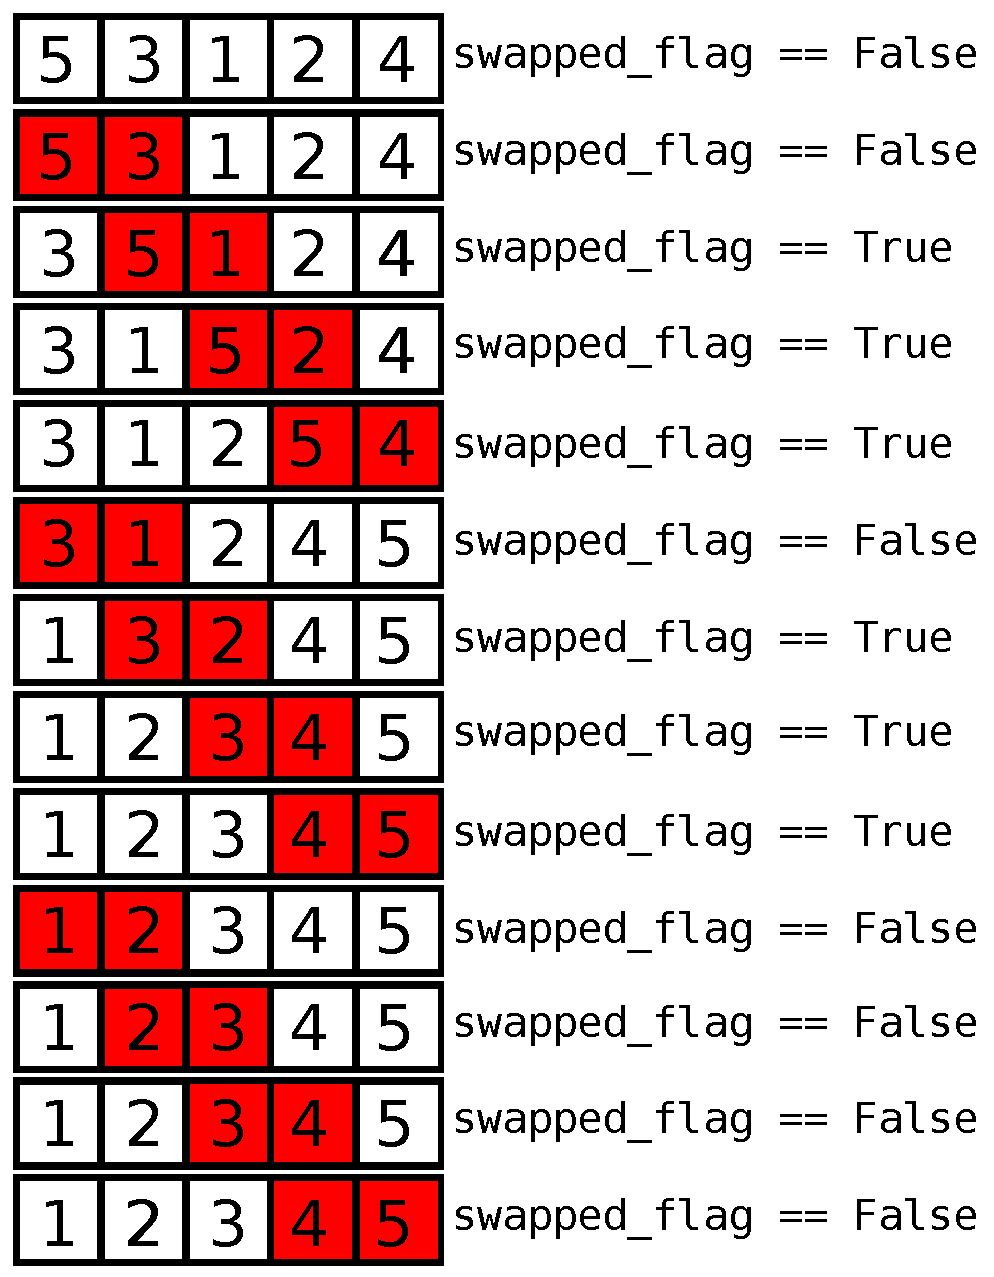
\includegraphics[width=0.8\linewidth]{Graphics/bubble_sort.pdf}
\caption{Schematic of Bubble Sort on a list.}
\label{fig_bubble_sort}
\end{figure}
\end{document}